%\documentclass[10pt,conference]{IEEEtran}
%\documentclass[9pt,conference]{sig-alternate}
%\documentclass[9pt,conference]{sig-alternate}
%\documentclass[10pt,print,letterpaper,nocopyrightspace]{sigplan-proc-varsize}
\documentclass[10pt,print,letterpaper]{sigplan-proc-varsize}

\usepackage{amsmath,epsfig}
\usepackage{url}
\usepackage{xspace}
\usepackage{colortbl}
\usepackage{subfigure}
\usepackage{dsfont}
\usepackage{boxedminipage}
\ifx\pdfoutput\undefined
\usepackage[hypertex]{hyperref}
\else
\usepackage[pdftex,hypertexnames=false]{hyperref}
\fi

\usepackage{amssymb}
\usepackage{wasysym}
\usepackage[left=2.54cm,top=2.54cm,right=2.54cm,bottom=2.54cm,nohead,nofoot]{geometry}



\DeclareMathOperator*{\argmax}{argmax}
%\usepackage{times}

\def\ucb{$^{\dagger}$}
\def\stanford{$^{\ddagger}$}
\def\arch{$^{\star}$}

\newcommand{\kb}{kB}
\newcommand{\rene}{Ren{\'e}\xspace}
\newcommand{\reneii}{Ren{\'e}2\xspace}
\newcommand{\wec}{WeC\xspace}
\newcommand{\mica}{Mica\xspace}
\newcommand{\micaii}{Mica2\xspace}
\newcommand{\micaz}{MicaZ\xspace}
\newcommand{\micadot}{Mica2Dot\xspace}
\newcommand{\iic}{I$^2$C\xspace}
\newcommand{\uA}{$\mu$A\xspace}
\newcommand{\dotmote}{Dot\xspace}
\newcommand{\mhz}{MHz\xspace}
\newcommand{\ghz}{GHz\xspace}
\newcommand{\kbps}{kbps\xspace}
\newcommand{\dsn}{DSN\xspace}
\newcommand{\io}{I/O\xspace}
\newcommand{\telos}{Telos\xspace}

\newcommand{\T}{\mathds{T}}
\newcommand{\XXXnote}[1]{{\bf\color{red} XXX: #1}}


\begin{document}

%\conferenceinfo{Sensys'08,} {November 5--7, 2008, Raleigh, NC, USA.}  
%\CopyrightYear{2008} 
%\crdata{978-1-60558-096-8/08/09} 

\title{StreamFS}
%\numberofauthors{1} 
%\author{\alignauthor Stephen Dawson-Haggerty, Jorge Ortiz, Xiaofan Jiang and David Culler\\
%\affaddr{Computer Science Division}\\
%\affaddr{University of California, Berkeley} \\ 
%\affaddr{Berkeley, California 94720} \\
%\email{\{stevedh,jortiz,xjiang,culler\}@cs.berkeley.edu}
%} 


%\subtitle{Paper \# Insert Reg Number Here}

%\title{Alternate {\ttlit ACM} SIG Proceedings Paper in LaTeX
%Format\titlenote{(Produces the permission block, and
%copyright information). For use with
%SIG-ALTERNATE.CLS. Supported by ACM.}}
%\subtitle{[Extended Abstract]
%\titlenote{A full version of this paper is available as
%\textit{Author's Guide to Preparing ACM SIG Proceedings Using
%\LaTeX$2_\epsilon$\ and BibTeX} at
%\texttt{www.acm.org/eaddress.htm}}}
%
% You need the command \numberofauthors to handle the 'placement
% and alignment' of the authors beneath the title.
%
% For aesthetic reasons, we recommend 'three authors at a time'
% i.e. three 'name/affiliation blocks' be placed beneath the title.
%
% NOTE: You are NOT restricted in how many 'rows' of
% "name/affiliations" may appear. We just ask that you restrict
% the number of 'columns' to three.
%
% Because of the available 'opening page real-estate'
% we ask you to refrain from putting more than six authors
% (two rows with three columns) beneath the article title.
% More than six makes the first-page appear very cluttered indeed.
%
% Use the \alignauthor commands to handle the names
% and affiliations for an 'aesthetic maximum' of six authors.
% Add names, affiliations, addresses for
% the seventh etc. author(s) as the argument for the
% \additionalauthors command.
% These 'additional authors' will be output/set for you
% without further effort on your part as the last section in
% the body of your article BEFORE References or any Appendices.

\numberofauthors{2} %  in this sample file, there are a *total*
% of EIGHT authors. SIX appear on the 'first-page' (for formatting
% reasons) and the remaining two appear in the \additionalauthors section.
%
\author{
% You can go ahead and credit any number of authors here,
% e.g. one 'row of three' or two rows (consisting of one row of three
% and a second row of one, two or three).
%
% The command \alignauthor (no curly braces needed) should
% precede each author name, affiliation/snail-mail address and
% e-mail address. Additionally, tag each line of
% affiliation/address with \affaddr, and tag the
% e-mail address with \email.
%
% 1st. author
\alignauthor
%Prabal Dutta\\
%       \affaddr{Computer Science Division}\\
%       \affaddr{Univ. of California, Berkeley}\\
%       \affaddr{Berkeley, CA 94720}\\
%       \email{prabal@cs.berkeley.edu}
% 2nd. author
%\alignauthor
%David Culler\\
%       \affaddr{Computer Science Division}\\
%       \affaddr{Univ. of California, Berkeley}\\
%       \affaddr{Berkeley, CA 94720}\\
%       \email{culler@cs.berkeley.edu}
% 3rd. author
%\alignauthor
%Scott Shenker\\
%       \affaddr{Computer Science Division}\\
%       \affaddr{Univ. of California, Berkeley}\\
%       \affaddr{Berkeley, CA 94720}\\
%       \email{shenker@cs.berkeley.edu}
%}
Jorge Ortiz\\
       %\affaddr{Department}\\
	\affaddr{Computer Science Division}\\
       \affaddr{University of California, Berkeley}\\
       %\affaddr{City, State Zip}\\
       \email{jortiz@cs.berkeley.edu}
}


\maketitle

%\date{14 April 2007}
%\maketitle

% \begin{abstract}
% Despite the growing impact of climate change and energy prices, 
per-capita energy consumption is rising. Part of the problem is visibility. We do not 
have scalable means of observing our energy consumption patterns and determining how to optimize and reduce our
consumption.
Mobile smartphones present a unique opportunity to enable an energy view on the physical world. 
They can bridge the physical world, information infrastructure, and people
through a rich set of sensors, ubiquitous connectivity, and highly personal user interface. 
With QR codes as cheap tags on items and places in the physical world, the
camera becomes a portable scanner in your pocket, in addition to its
traditional functions.  We explore this
unique triple point
and re-examine classical problems of context and consistency management in mobile
systems.  We also examine this combination as it pertains to energy management of physical
devices.  In doing so, we are re-introduced to problems of apportionment and aggregation of sensor data,
except with a continuously changing set of constituents.  We describe our solution in a technique
called \emph{dynamic aggregation} that maintains moving aggregates as the
set of data sources changes over time.  We deployed our system in a 
141,000 square-foot building, tagging 351 items over 139 room across 7 floors.

% When combined with QR codes, the on-board camera provides us with a portable scanner

% The camera,
% when combined with QR codes, gives us a portable scanner and convenient mechanism for tying these world together. 
% In this paper, we describe our system and deployment experience for a mobile phone application the provides 
% user-centric energy-view of the physical world. We describe the challenges, specifically dealing with mobility, 
% and how we address them in a set of three separate applications: an energy auditing application, a 
% device energy scanner, and a personal energy counter. We also introduce a technique called \emph{dynamic aggregation}
% which allows us to seamlessly track the constituents of aggregated energy calculations, as they move from one 
% location to another.

% Despite the recent impact of global warming and a steady increase in energy prices, 
% per-capita energy consumption is rising. Part of the problem is about visibility. We simply do not 
% have any good ways of seeing how we consume energy, and therefore, how to optimize and reduce it. 
% \end{abstract}

% A category with the (minimum) three required fields
%\category{B.0}{Hardware}{General}
%\category{B.4}{Hardware}{Input/Output \& Data Communication}

%\terms{Design, Implementation, Performance, Experimentation}

%\keywords{Churn, Link, Routing, Wireless, Sensor Network, Mote}

%\newpage
% \subsection{Introduction}
The United States leads the world in per-capita energy consumption.
Our electricity use has consistently increased over the last 40 years~\cite{oecd2011} and other parts of the world are rising all 
too rapidly.  With the specter of climate change and the increasing cost of energy, we must explore new
ways for individuals to gain visibility and insight into their energy consumption in order to optimize and reduce it. 
With the increasing penetration of embedded sensors in the environment and
the continued rise in smartphone adoption, we see an opportunity for smartphones to bridge the physical world
to our computational infrastructure and provide an `energy lens' on the physical world.  

We use mobile phones to construct an entity-relationship 
graph of the physical world and combine it with streaming sensor data in order to perform detailed energy-attribution.
We limit the scope of the world to a single building domain.  We have designed and implemented a real-time, mobile energy auditing
application, called the `Energy Lens', that allows us to collect information about 
things throughout the building and how they are related to each other.  For example, computer X is inside 
room Y and connected to meter Z.  Then, we use these relationships to guide our data look-up and analytical
calculations.  For example, the load curve of room Y consists of the sum of all the power traces for loads
inside room Y.  We use the mobile smartphone as the main input tool.  Our work examines \emph{three main challenges} in setting up and 
deploying a real, whole-building infrastructure to support real-time, 
fined grained energy analytics.  

The first challenge is related to tracking and mobility.
The use of mobile phones presents classical, fundamental challenges related to mobility.  Typically, mobility
refers to the phone, as the person carrying it moves from place to place.  However, in the energy-attribution
context, we are also referring to the movement of energy-consuming objects.  Tracking their relationships to spaces 
and people is as important as tracking people.  We describe how we deal with \emph{both moving people and 
moving objects} and show that these historically difficult problems can be addressed relatively easily, if the proper infrastructure is 
in place.  %We provide evidence that the approach is simple, incrementally deployable, and scalable.

The second challenge is about capturing the inter-relationship semantics and having these inform our  analytics.
We adopt the general notion of physical tags that identify objects in the world.  Our system uses \emph{QR codes} to tag things and locations 
in the physical world.  However, \emph{any tag that provides a unqiue identifier for an object could serve the same purpose}.
Once tagged, there are three types of interactions -- 
registration, linking, and scanning -- which establish important relationships.  Registration is the act of creating a virtual object 
to represent a physical one.  Linking captures the relationship between pairs of objects.  Scanning is the act of performing an item-lookup.
Each of these interactions requires a set of swiping gestures.  Linking requires two tag swipes while the other two actions
require a single tag swipe.  Internally, we maintain a \emph{entity-relationship graph (ERG)} of things, people, and locations, that gets
updated through these sets of gestures.

The third challenge is about indoor network connectivity and access.
In order to connect these components, we rely on having `ubiquitous' network connectivity.  However, in practice, network
\emph{availability} is intermittent and our system must deal with the challenges of intermittency.  We discuss how caching
and logging are used to address these challenges.  Moreover, when connectivity is re-established, we must deal with
applying updates to the ERG, as captured by the phone while disconnected.  
% Conflicts can also occur during an update.  For example, the two updates may disagree about which items are attached
% to which meters.  We implement a very simple conflict resolution scheme, described in section~\ref{sec:conflicts}.
% Finally, certain physical-state transitions are represented as a set of updates to the ERG that must be applied 
% atomically.  We implement transactions in the log-replay and transaction manager.
% Our `Energy Lens' system is deployed in a building on our campus.  We discuss
% its architecture and our design choices.  
  
% We also discuss novel strategies for tracking moving people/things and describe how we implement these in our system.  In summary, our work
% makes the following contributions:

% \begin{itemize}
% \item We design and implement a system that captures and combines physical entities, their inter-relationships, and real-time sensor data 
% 		in buildings.% using mobile phones, qr code, and a cloud-based infrastructure.
% \item We observe that certain combinations of swipes give us useful information to set the location of people and things over time.
% 		We codify this observation in our \emph{context-tracker} and use it to maintain consistency between the entity-relationship graph and the 
% 		state of the physical world.  To the best of our knowledge, this is radically different from the approaches in standard 
% 		localization techniques.  However, we argue that it can be used to \emph{enhance} their accuracy and overall performance.
% \item We implement a prefetching algorithm to obtain context-dependent information to both improve performance and
% 		enable disconnected operation.  We also design and implement a log-replay and transaction manager over our data management layer.  We describe how different conflict-resolution policies can be implemented and our rationale for the policies we chose.
% \end{itemize}

% \vspace{0.08in}

% In the next sections we go through a motivating scenario.  We then discuss some related work, followed 
% by the system architecture, evaluation, and future directions.


%
% The marriage of pub/sub, streaming dbms, and filesystems
%

\subsection{Introduction}
The United States leads the world in per-capita energy consumption.
Our electricity use has consistently increased over the last 40 years~\cite{oecd2011} and other parts of the world are rising all 
too rapidly.  With the specter of climate change and the increasing cost of energy, we must explore new
ways for individuals to gain visibility and insight into their energy consumption in order to optimize and reduce it. 
With the increasing penetration of embedded sensors in the environment and
the continued rise in smartphone adoption, we see an opportunity for smartphones to bridge the physical world
to our computational infrastructure and provide an `energy lens' on the physical world.  

We use mobile phones to construct an entity-relationship 
graph of the physical world and combine it with streaming sensor data in order to perform detailed energy-attribution.
We limit the scope of the world to a single building domain.  We have designed and implemented a real-time, mobile energy auditing
application, called the `Energy Lens', that allows us to collect information about 
things throughout the building and how they are related to each other.  For example, computer X is inside 
room Y and connected to meter Z.  Then, we use these relationships to guide our data look-up and analytical
calculations.  For example, the load curve of room Y consists of the sum of all the power traces for loads
inside room Y.  We use the mobile smartphone as the main input tool.  Our work examines \emph{three main challenges} in setting up and 
deploying a real, whole-building infrastructure to support real-time, 
fined grained energy analytics.  

The first challenge is related to tracking and mobility.
The use of mobile phones presents classical, fundamental challenges related to mobility.  Typically, mobility
refers to the phone, as the person carrying it moves from place to place.  However, in the energy-attribution
context, we are also referring to the movement of energy-consuming objects.  Tracking their relationships to spaces 
and people is as important as tracking people.  We describe how we deal with \emph{both moving people and 
moving objects} and show that these historically difficult problems can be addressed relatively easily, if the proper infrastructure is 
in place.  %We provide evidence that the approach is simple, incrementally deployable, and scalable.

The second challenge is about capturing the inter-relationship semantics and having these inform our  analytics.
We adopt the general notion of physical tags that identify objects in the world.  Our system uses \emph{QR codes} to tag things and locations 
in the physical world.  However, \emph{any tag that provides a unqiue identifier for an object could serve the same purpose}.
Once tagged, there are three types of interactions -- 
registration, linking, and scanning -- which establish important relationships.  Registration is the act of creating a virtual object 
to represent a physical one.  Linking captures the relationship between pairs of objects.  Scanning is the act of performing an item-lookup.
Each of these interactions requires a set of swiping gestures.  Linking requires two tag swipes while the other two actions
require a single tag swipe.  Internally, we maintain a \emph{entity-relationship graph (ERG)} of things, people, and locations, that gets
updated through these sets of gestures.

The third challenge is about indoor network connectivity and access.
In order to connect these components, we rely on having `ubiquitous' network connectivity.  However, in practice, network
\emph{availability} is intermittent and our system must deal with the challenges of intermittency.  We discuss how caching
and logging are used to address these challenges.  Moreover, when connectivity is re-established, we must deal with
applying updates to the ERG, as captured by the phone while disconnected.  
% Conflicts can also occur during an update.  For example, the two updates may disagree about which items are attached
% to which meters.  We implement a very simple conflict resolution scheme, described in section~\ref{sec:conflicts}.
% Finally, certain physical-state transitions are represented as a set of updates to the ERG that must be applied 
% atomically.  We implement transactions in the log-replay and transaction manager.
% Our `Energy Lens' system is deployed in a building on our campus.  We discuss
% its architecture and our design choices.  
  
% We also discuss novel strategies for tracking moving people/things and describe how we implement these in our system.  In summary, our work
% makes the following contributions:

% \begin{itemize}
% \item We design and implement a system that captures and combines physical entities, their inter-relationships, and real-time sensor data 
% 		in buildings.% using mobile phones, qr code, and a cloud-based infrastructure.
% \item We observe that certain combinations of swipes give us useful information to set the location of people and things over time.
% 		We codify this observation in our \emph{context-tracker} and use it to maintain consistency between the entity-relationship graph and the 
% 		state of the physical world.  To the best of our knowledge, this is radically different from the approaches in standard 
% 		localization techniques.  However, we argue that it can be used to \emph{enhance} their accuracy and overall performance.
% \item We implement a prefetching algorithm to obtain context-dependent information to both improve performance and
% 		enable disconnected operation.  We also design and implement a log-replay and transaction manager over our data management layer.  We describe how different conflict-resolution policies can be implemented and our rationale for the policies we chose.
% \end{itemize}

% \vspace{0.08in}

% In the next sections we go through a motivating scenario.  We then discuss some related work, followed 
% by the system architecture, evaluation, and future directions.


\section{Physical-data applications}
Physical-data applications are applications built to provide insight about the physical world.  They range from
analytics and visualization to control and actuation.  Analytics and visualization apps typically 
provide aggregates, statistical summaries, and future predictions about the behavior of the physical phenomenon 
being measured.  The fundamental challenges for these application are dealing with flawed or missing sensor data,
integrating smoothing and processing models to fill in gaps in the data, and maintaining consistency
between the physical world and the representation of it within the processing system, particular as it evolves.  
\emph{Context maintainence} is a fundamental challenge for correct interpretation of the physical data.

Control applications allow users to control their environment.  Control applications are either built off
analytics, providing intelligent, model-based control or they can provide simple, local, direct actuation by users 
through item or context-specific user interfaces.

Security is also a major concern in physical-data applications.  Physical data reveals personal information
about users through their affect on physical measurements.  For example, light sensors and location information
indicates occupation.  Energy-consumption aggregates, when grouped by user or localtion can give information about
the energy consumption habbits the occupants or users of those spaces.

\subsection{Data organization, data services}
\subsection{Context consistency maintenance}
\subsection{Dashboards}
\subsection{Analytics}
\subsection{Control}

\section{Subscription semantics}
A subscription expresses the intent to receive all associated streams whose topic is expressed by its hardlink name
or any associated alias.  Fundamentally, the subscriber expresses an interest in specific streams, referred to
directly by name or indirectly by topic matching as it pertains to regular-expression name matching.

\subsection{Continuous group-by for aggregation}
Many of the application queries require aggregation of data over groups of streams.  However, membership to those groups
change over time, so aggregate recalculation must account for the changing constituents in order to maintain accuracy.
Because of the way subscriptions are implemented in StreamFS, this is handled automatically.  Recall, only 
streams whose tags match a subscriber's regular expression is forwarded to the subscription target.  By removing 
a tag, you change group membership.  Tag removal \emph{can} change the membership of a stream to a group of streams
defined by the regular expression.  The data from streams belonging to the group are no longer accounted for in the aggregate
calculation.  The same is true when new members join the group.  Aggregate calculation accuracy is maitained
in either case.

Lets go through an example.

\begin{figure}
\centering
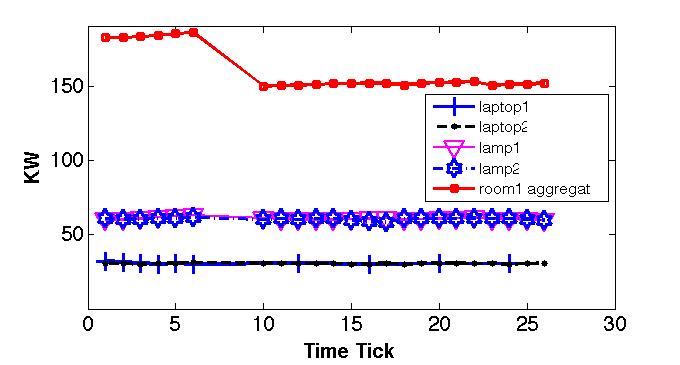
\includegraphics[width=.45\textwidth]{figs/dynagg_scenario1_room1.png}
\caption{}
\label{fig:dynagg}
\end{figure}


\section{Stream processing}
StreamFS allows users to perform stream processing on collections of streams.

Preserving timing semantics is challenging for two reasons:

\begin{enumerate}
\item NodeJs is single threaded; although it's an implementation issues, it's clear that
the scheduler can only handle one job at a time, so threading is necessary
\item load is a metric of cpu activity, but the real metric we care about is expected versus
actual start and completion time of a job.
\end{enumerate}

The second point is the important factor that determines when a job gets moved to another server.
We aim to maximize CPU utilization on a single server, without sacrificing timing constraints specified
by the user.  Job execution timing quality is measured by the absolute deviation of the completion
time of a job from the scheduled completion time, that quality measure degrades as computing cycles
become more scarce.  In other words, the less cpu cycles there are to schedule the CPU-bound job, the
larger the average error and variance of job completion times.

Now I have to show this experimentally and describe the methodology and job scheduling/migration algorithm.

% \subsection{Job scheduling and migration}
% Lets assume we have a job $J$ that takes $T_{c}$ to complete is scheduled to run every $T_{p}$ seconds. 



\section{Processes Job Scheduling}
Lets assume we have a job $J$ that takes $T_{c}$ to complete is scheduled to run every $T_{p}$ seconds. 


\section{Process and sample scheduling}
A job specifies both the report period and timeout time.  The job also specifies, implicitly or
explicitly, which sensor streams will be consumed.  These parameters are used by the process manager
for scheduling those streams such that 1) we maximize the number of jobs that make use of a report
and 2) we minimize the error introduced by waiting for a report; interpolating later in time, introducing
more error.  The former keeps the CPU more highly utilized doing active work, the latter allows jobs to 
run on the freshest data (or its closest approximation).  

The driver has two reporting modes.  The first is for sensors whose report period can be set
and the other is for those whose report period cannot be set.  The driver decouples the report
capabilities of the underlying hardware from the report mechanism to the process manager.  This 
allows for scheduling flexibility in the process
manager.  We argue that this is a critical design choice, for processing efficiency, when dealing 
with the integration of heterogenous physical data streams.  In addition, we embedded a simple linear
interpolation process in the driver code itself.  This gives the scheduler flexibility in choosing the
data value from the sensor for timestamp alignment with the other sensors.  We observe that readings,
in close temporal proximity, are linearly associated with prior readings; especially as
the temporal distance decreases.

Jobs in the system specify a maximum report period of the job and the $k$ streams it consumes.  
Data streams fall into two categories: those that can be scheduled and those that cannot.  For
those that can be scheduled the questions are how do we \dots

\begin{enumerate}
\item schedule their report periods such that each job as the minimum number of data points per stream in 
less than the maximum report period for that job?
%\item schedule their report period to maximize overlap with the job report period?
%\item schedule their report period to minimize the wait time between the actual reading and the report time?
\end{enumerate}

By default, drivers linearly interpolate pairs of readings.  We assume, for simplicity, that
1) a reading contains no error and 2) the longer we wait, the larger the error.  The 
error is proportional to the amount of time since the last reading, times a constant.
The constant is stream specific.  We capture this, using a stream-specific weight constant.
For streams that cannot be scheduled, we ask, how do we \dots

\begin{enumerate}
\item set their report periods such that the time distance between the interpolated (reported) value
and the raw (actual) value is minimized across all $k$ streams.
\end{enumerate}

\subsection{Sample scheduling}
There are $n$ jobs, each with a period $P_{i}$ for some job $j_{i}$.  Each stream, $j_{i}$, consumes a set
of streams $K_{i}$.  A job also specifies the minimum number of data points necessary from each stream.
In this scenario, each stream $s \in K_{i}$ can be scheduled with any period $p$
and start time, $t_{init}$.  For our jobs, we can stop and re-start them to get them to re-align after
a scheduling decision has been made.  The goal is to meet the maximum deadline while providing each job
the number of necessary data points from each stream.


\subsubsection{Variable Sensing Schedule}

\subsubsection{Fixed Sensing Schedule}
Let $t_{i}$ be the  next time the job will run.


\subsubsection{Error Minimization}

\section{Mixed Strategy}









\subsection{Experimental results}


\section{Filesystem for streaming data}
% Files provide an abstraction over collection of bytes on disk.  The file provides an interface where
% bytes are disk are logically sequential, allowing applications to refer to collections of bytes given an
% offset and length.  In the traditional case, bytes are physically distributed throughout the disk.  As data
% is read/written from the file, it is done so relative to the starting byte of the file, sequentially.
% In a sense, the file abstraction is convenient for dealing with distributed data.  Although (in most cases)
% locally on disk, sequential access interfaces for the application make it easier to browse, edit, 
% and acess the information without thinking about where the bytes are actually laid out.

% In a similar sense we think that interface can also serve as a convenient access abstraction.  Timeseries
% data gives us

A file system provides an abstraction for managing a collection of bytes on disk.  The standard file itself
provides logically sequential access to bytes distributed through the disk.  Directories provides a simple
container mechanism for grouping together files that are in some way related to each other.  We think deployment
metadata and data can similarly benefit from a simple hiearchical naming structure.  Grouping items that share
overlapping name-elements separated by forward-slashes in their tags.  It provides a simple
way to specify groups of streams as the unit of access or processing.  File systems have also developed
a convenient set of tools for quickly locating information, sharing reading, and pipelining processing; simple
tools that fit the access, sharing, and processing needs for local-area sensor deployments.  Filesystem also
provide a security model baked into their construction.  We examine the filesystem interface to StreamFS and 
examine how well the interface fits the needs for the class of applications StreamFS supports.


\subsection{Naming and access}
For local-area deployments, where spatial or categorical referral patterns are common in the tagging structure, 
hierarchical grouping provides a good, simple fit for naming objects.  However, we separate logical grouping from physical, 
and by doing so, also separate naming and access.  This prevents overly-stringent access patterns that may degrades 
performance over time.  How the data is accessed is independent of how the object named.  It also support multiple names without
affecting without affecting access.

Tags are abitrary, but forward-slash separated naming conventions map cleanly into a filesystem naming.  Each 
string between the forward slashes is treated like a directory in the filesystem.  If a user attempts to 
create a file with an element in the name that is already set for a non-container object in StreamFS, then creation
of the file is not allowed.

\subsection{File types: directories, regular, special, pipes}

\subsection{Filesystem tools: grep, find, ls}

\section{Publish/subscribe model}
Eugster et al.~\cite{eugster}.

StreamFS uses a flexible flavor of the publish/subscribe model in order to support a wide range of applications.  
Publish/subscribe is necessary is physical data application development in order to scale in the number of supported
applications.  The publish/subscribe model used in StreamFS provides mechanisms that enable a flexible combination 
of space and time decoupling that enable StreamFS to support of a wide arrange of application requirements.

Our pub/sub engine is also tightly coupled with the namespaces expose to users, and this design choice allows an application
to control the space coupling between the publisher and the subscriber (similar to TIBCO~\cite{tibco}).

\subsection{Space decoupling}
By its very design, space decoupling is achieved.  Publisher do not hold a reference to the subscriber and subscribers do not
hold references to publisher.  However, because of the coupling of a full pathname and an object, subscriptions to topics
expressed as a full pathname refer to the single publisher.

\subsection{Time decoupling}
Time decoupling is achievable through the timeseries data store.  Publisher push data to StreamFS whether or not subscribers are
online.  Moreover, data may be received at the subscriber even if the publisher becomes disconnected.  Currently, subscribers do
not receive all information that was missed.  In order to achieve fill time-decoupling, we allow the subcription
target to enable or disable the option to buffer all missed readings for an associated subscription target, while the subscription
target it offline.

\subsection{Synchronization decoupling}
Sychronization decoupling is achieved by the publisher and subscribers through StreamFS.  Events are received out of sequence
from their arrival to StreamFS.  This is true even when the subscription target is a processing element.  The thread that buffers
incoming data for each processing element is seperate from the thread where the process is executed.

\section{Security}

\subsection{Confidentiality}
With SSL over Https for rest interface.
With SSL flat over standard sockets.

\subsection{Authentication}
Public-private key encryption used for authentication: \\
$A \rightarrow Msg(Username, Public\_key\_A) \rightarrow B$ \\
$A \leftarrow Msg(Enc\_Pub\_A(APP\_ID)) \leftarrow B$ \\

\begin{enumerate}
% \item Over regular socket: set auth=on, body should include $Enc\_Priv\_A(username, APP\_ID, msg)$ as POSTed data
% 	\begin{itemize}
% 	\item this provides confidentiality and authentication
% 	\end{itemize}
\item Logging in should be an done over a secure socket and include the ``username'' and ``password'' of the user.  If 
		successful, the server will return an ``sid'' that has a TTL of 24 hour idle time.

\item Over secure socket ``query\_params'' in json object (or query parameters in the https request) should 
		include the ``sid'' (session identifier), returned from the server after sucessfully logging in a creating a new session.\\	
	\begin{itemize}
	\item confidentiality provided by secure socket layer
	\item the ``sid'' provides a ticket for a previous successful login.
	\end{itemize}

\end{enumerate}

The key is that we want to determine who is making the request so we can determine whether to satisfy that request.

\subsection{Access control and privacy}
ACLs.  (Username, APP\_ID)

Users can create various applications, giving each application a unique identifier.  This allows users to share
data explicitly between applications.  There are 5 levels of access:
\begin{enumerate}
\item Group: groups of (users,application) tuples
\item User: identified by (name, public key)
\item application
\item resource
\item operation (read/get, write/post,put, execute/put,post)
\end{enumerate}

Application boundaries are useful for separating data-only (read/write only data) application from control applications.
For example, we have one application that wants to display the total energy consumed by the lights in the building and 
it even writes the aggregate light energy consumption data to a resource and makes that resource available.  The light-control
application also read data coming from the lights through resources owned by the light data application, but it produces
information about how it's controlling the light accordingly that it does not want other application to view. 
In this case the light data app shares its resources with the light control app, but not the other way around, even though
both apps were written by the same user.  In addition, the user is relieved from managing which collections of resources
should not be read by the light-data app, resting assured that anything owned by the control app is not accessible by
the light-data app.


\vspace{+0.5mm}
\vspace{+2mm}
\bibliographystyle{abbrv}
%\scriptsize
\bibliography{references}

\end{document}


